\part{A PROPOSTA DE TRABALHO}

\chapter[A Proposta de Trabalho]{A Proposta de Trabalho}

\section[Definição da Proposta]{Definição da Proposta}

Neste trabalho foi apresentado uma série de leis, instruções normativas e acórdãos pertinentes à contratação de serviços de TI e foram apresentados também os principais conceitos do Pensamento Lean, Kanban e de Metodologias Ágeis. Toda a informação apresentada neste trabalho será importante para o entendimento e aplicação da proposta deste estudo de caso.

Dentro da legislação pertinente a contratação, foi selecionada como foco deste trabalho a fase de Gerenciamento do Contrato do Modelo de Contratações de Soluções de TI apresentando pela Instrução Normativa nº 04. Das metodologias, será utilizada como foco deste trabalho a análise da aplicação do Kanban, advindo do Lean,  e do Scrum em uma instituição pública brasileira. 

Ao analisar trabalhos que já foram desenvolvidos, não foram encontrados estudos que buscassem sistematicamente levantar e analisar os aspectos advindos do uso de uso de metodologias ágeis em contraposição ao uso de metodologias tradicionais na gestão de contratos de fornecedores de desenvolvimento de software.

Assim, proposta deste trabalho consiste no levantamento de dados passados de contratações de fornecedores de desenvolvimento de software por uma instituição pública brasileira para fim de comparação entre os resultados obtidos com uso de metodologias ágeis e os resultados obtidos sem o uso das metodologias ágeis na gestão de contratos de fornecedores de desenvolvimento de software.Com este objetivo, será realizado um estudo de caso que será definido na próxima seção.


\section[Estudo de Caso]{Estudo de Caso}

Nesta seção será apresentada a proposta de realização de um estudo de caso na área de TI de um órgão público federal brasileiro, sendo esta uma forma de aplicar os conhecimentos adquiridos ao longo do trabalho e de coletar dados da experiência do órgão tanto em gestão de contratos com métodos ágeis quanto em gestão de contrato com métodos tradicionais.

O órgão público selecionado foi o Instituto do Patrimônio Histórico e Artístico Nacional (IPHAN).

O escopo do estudo de caso está ilustrado na figura 17. 
\begin{figure}[H]
		\centering
		\label{fig01}
			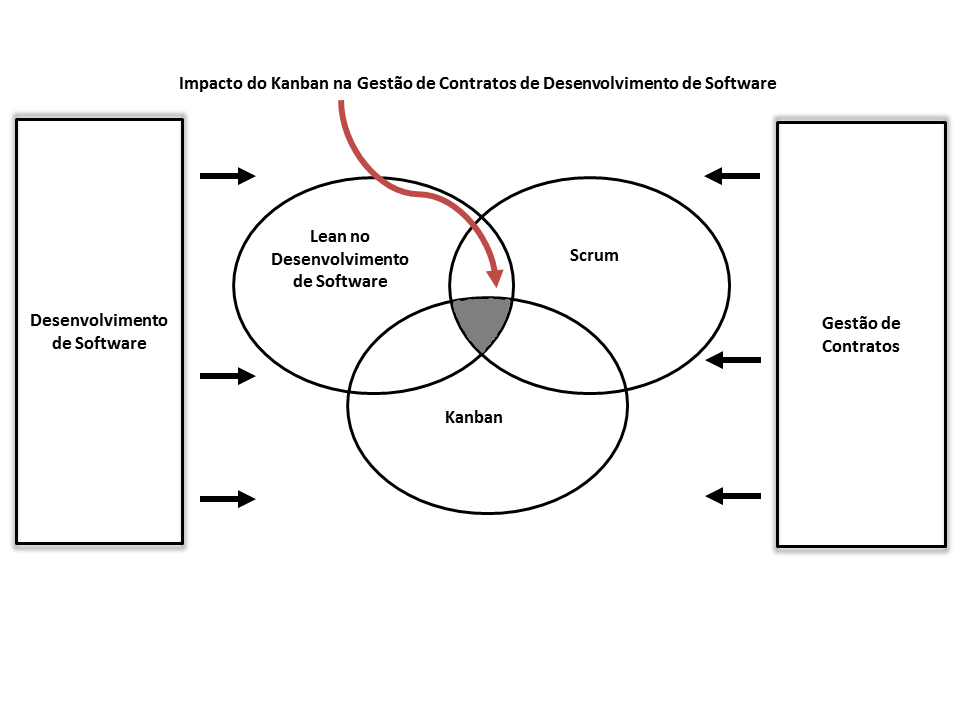
\includegraphics[scale=0.6]{figuras/escopoEC.png}
		\caption{Escopo do Estudo de Caso}
\end{figure}

\subsection[A Organização]{A Organização}

O órgão escolhido, IPHAN, possui uma força de trabalho atuante na área de TI de apenas 8 funcionários, dos quais apenas 3 trabalham diretamente com sistemas e um deles é o responsável pela gestão de demandas. Os contratos mais significantes gerenciados pela área de TI do órgão são:
\begin{itemize}
\item Demanda para desenvolvimento de sistemas (sistema novo, manutenção, documentação ou refatoração).
\item Demanda de controle de qualidade de sistemas.
\item Demanda de medição de sistemas.
\end{itemize}

Devido ao o número reduzido de servidores disponíveis na área de TI do órgão, muitas vezes uma só pessoa pode desempenhar mais de um dos papéis definidos na IN 04. Além disso diversos problemas começaram a ser identificados com o uso de metodologias tradicionais, dentre eles:
\begin{itemize}
\item Não entrega de software.
\item Pagava apenas por documentação.
\item Dificuldade para aferir a qualidade interna do produto.
\item A mudanças tardias geravam grande impacto no tempo de execução do projeto.
\end{itemize}

O contexto atual do órgão foi identificado por meio da aplicação da técnica de entrevista semi-estruturada. A estrutura da entrevista pode ser encontrada no Apêndice I -  Roteiro de Entrevista.  Com os problemas que foram identificados, as principais motivações para o uso de metodologias ágeis na gestão de contratos foram: entregar mais software, pois o órgão nunca tinha tido um contrato com completo sucesso, e poder perceber de forma mais rápida se o projeto terá sucesso ou não, pois os riscos inerentes à contratação poderiam ser identificados mais previamentes.

Pela pesquisa documental identificou-se que o órgão possuí uma Metodologia de Gestão de Demandas de Desenvolvimento de Software, detalhada no Anexo B, e um Kanban para Gestão de 
Demandas, o qual foi apresentado no capítulo anterior. 

Segundo a IN 04 a fase de Gerenciamento de Contrato deve conter seguintes etapas: início do contrato; encaminhamento formal de ordem de serviço ou fornecimento de bens  monitoramento da execução; e transição contratual e/ou encerramento do contrato. Todas estas etapas podem ser observadas na metodologia definida pelo órgão, fazendo com que ele seja aderente a legislação e adequado para o estudo de caso deste trabalho.

Segundo um representante do órgão, as metas definidas para a construção da metodologia de gestão de demandas foram:
\begin{itemize}
\item Ser aderente à legislação pertinente.
\item Entregar software mais rapidamente.
\item Focar na gestão do contrato e na definição de uma metodologia de gestão de demandas.
\item Não focar em dizer como a empresa deve desenvolver o software, ou seja, não definir metodologia de desenvolvimento de software.
\item Satisfazer as necessidades do cliente.
\end{itemize}

Outro aspecto que foi tratado de forma diferente com o uso de metodologias ágeis na gestão de contratos foi a forma de pagamento e a aplicação de multas. Diferente das outras formas de gestão de contrato onde existem diversas categorias para aplicação de multas, que variam de acordo com diversas variáveis como tipos de erros ou dias de atraso, com o uso de métodos ágeis na gestão do contrato os pagamentos eram feitos a cada entrega (Sprint) em curtos intervalos de tempo, o que mantinha o fluxo de caixa da empresa contratada sempre ativo, e as multas eram somente aplicadas se nada fosse entregue, se algo fosse entregue de forma incompleta não era aplicada multa, pois há o bom senso que a empresa ainda está adquirindo maturidade no contrato, e se o que foi entregue tivesse erros ou não estava conforme o que foi pedido era feito um abatimento no pagamento.

De forma geral, o órgão começou a notar alguns benefícios com a aplicação de métodos ágeis, em especial o Kanban, na gestão de contratos, dentre os principais estão: visibilidade para o gestor do negócio (cliente) sobre o que estava sendo feito, o domínio do gestor do negócio sobre a gestão do Backlog, definindo quais seriam as próximas funcionalidades a serem desenvolvidas, e o gestor do contrato passou a ser responsável somente pela gestão dos contratos e não mais por gerenciar requisitos e desenvolvimento de software.


\subsection[Questões de Pesquisa]{Questões de Pesquisa}

Neste estudo de caso serão analisadas questões dentro do contexto escolhido a fim de verificar a eficiência do uso de métodos ágeis e do Pensamento Lean, principalmente, por meio do Kanban no gerenciamento de contratos de fornecedores de desenvolvimento de software. Para isso, serão selecionados contratos para análise das questões de pesquisa a seguir definidas. As questões de pesquisa definidas foram:
\begin{itemize}
\item  A utilização de Metodologias Ágeis combinadas com o Lean Software na gestão de contratos aumenta a quantidade de contratos que são finalizados com sucesso?
\item  A utilização de Metodologias Ágeis combinadas com o Lean Software na gestão de contratos diminui o tempo para entrega de software?
\item	A satisfação do cliente com o resultado da contratação é maior com a utilização de Metodologias Ágeis combinadas com o Lean Software na gestão de contratos?
\item  O custo final do contrato no que diz respeitos às horas de trabalho dos servidores que são pagas é menor com a utilização de Metodologias Ágeis combinadas com o Lean Software na gestão de contratos?
\item  O processo para autorização de uma mudança no software leva menos tempo com a utilização de Metodologias Ágeis combinadas com o Lean Softwarena gestão de contratos?
\item	A quantidade de multas aplicadas na gestão de contratos é menor com a utilização de Metodologias Ágeis combinadas com o Lean Software?
\item	A quantidade de documentação desnecessária entregue para o gestor do contrato e para o órgão é menor com a utilização de Metodologias Ágeis combinadas com o Lean Software?
\item  A qualidade do produto gerado com a utilização de Metodologias Ágeis combinadas com o Lean Software na gestão de contratos é maior?
\end{itemize}

\subsection[Fonte e Método Coleta de Dados]{Fonte e Método de Coleta de Dados}

Os dados serão coletados por meio de entrevistas semiestruturadas e por meio da análise de documentos de cerca de quatro contratos que serão disponibilizados pelo órgão. Os contratos disponibilizados serão:
\begin{itemize}
\item  O contrato do Sistema Integrado de Conhecimento e Gestão (SICG) com a empresa EGL - Engenharia, no qual foram utilizadas metodologias ágeis para gestão do contrato.
\item  O contrato do Fiscalis com a empresa Velp Tecnologia, no qual foi utilizado o MPS-BR como base da gestão do contrato.
\item  O contrato do SIGIPHAN com a empresa Gestão TI, no qual não foi utilizado qualquer metodologia na gestão do contrato.
\item  O contrato com a empresa Squadra que desempenhou o papel de fábrica de software, desenvolvendo projetos diversos, no qual foi utilizado o Rational Unified Process (RUP) para gestão do contrato.
\end{itemize}

\section[Resultados Esperados]{Resultados Esperados}

Neste trabalho espera-se ter como resultado uma análise comparativa entre o uso de metodologias ágeis, em especial o Kanban, e sem o uso destas metodologias na gestão de contratos de fornecedores de desenvolvimento de software baseada nas hipóteses definidas.

\section[Cronograma de Execução]{Cronograma de Execução}

O cronograma de marcos definido para atingir o objetivo deste trabalho com as atividades já desenvolvidas e com as atividades futuras é apresentado na figura 18. Estão apresentados  no cronograma os marcos deste trabalho e os marcos para o trabalho final a ser realizado no próximo semestre.

\begin{figure}[H]
		\centering
		\label{fig02}
			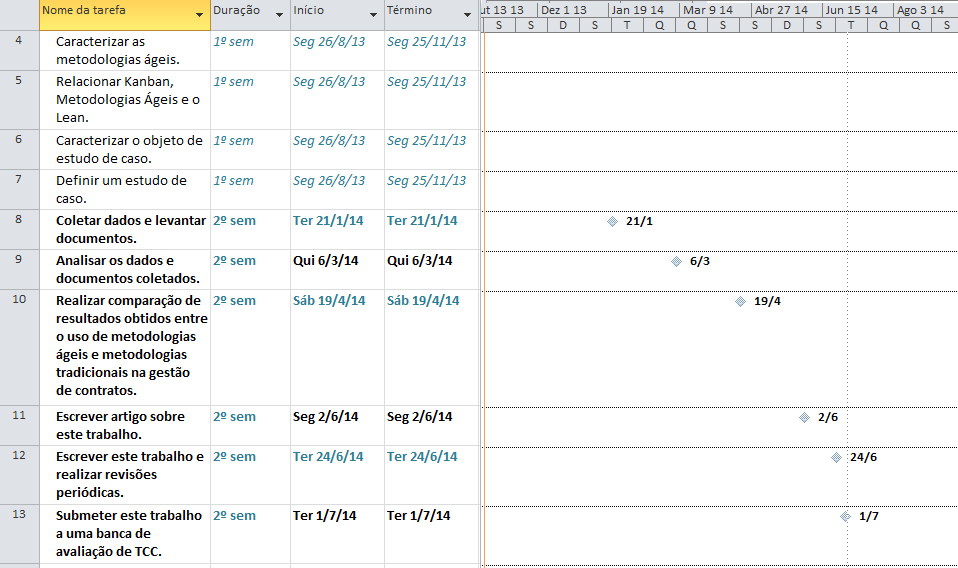
\includegraphics[scale=0.6]{figuras/cronograma2.png}
		\caption{Cronograma de Marcos}
\end{figure}
